\chapter{Consultas por similitud}
\hrule \bigskip \vspace*{1cm}


\section{Consideraciones iniciales}

En el área de base de datos, las técnicas de indexación tienen como objetivo auxiliar el almacenamiento y la recuperación eficiente de datos. Muchas de estas técnicas se aplican a tareas de recuperación de información. En general, la organización se lleva a cabo a través de una estructura de indexación, también denominado como Método de Indexación (MI) o Método de acceso (MA). Aplicaciones de base de datos emplean métodos de acceso como Métodos de Acceso Espacial (MAEs) y los Métodos de Acceso Métrico (MAM) debido a su capacidad para construir una estructura de datos para gestionar y organizar grandes cantidades de datos de manera eficiente.

Sin embargo, debido a la "maldición de la alta dimensionalidad'', el tiempo necesario para llevar a cabo la búsqueda por similitud, como kNN, puede crecer exponencialmente con la dimensionalidad de los datos. Aunque no se conoce ningún método para un buen desempeño en todas las instancias del problema, hay muchos algoritmos para acelerar las consultas, por lo general a través de una aproximación a la respuesta correcta. Así, se definen dos tipos de búsqueda: Métodos de búsqueda exactos y métodos de búsqueda aproximada; sobre los métodos de búsqueda de línea Búsqueda exacta de los métodos de acceso espacial (SAMs) y los métodos de acceso Métrico (MAM) son los más conocidos y utilizados en muchas aplicaciones.

La línea de investigación de los métodos de búsqueda exacta, los Métodos de  Acceso Espaciales (MAEs), como Kd-Tree \cite{kdt}, R-Tree \cite{Guttman1984}, R*-Tree \cite{rstartree}, R+-Tree \cite{rplustree}  y , X-Tree \cite{xtree}, describen los datos de entrada como vectores multidimensionales. Estos métodos fueron concebidos para apoyar las operaciones de búsqueda involucrando puntos y objetos geométricos.

Aunque en esta línea, Faloutsos \cite{GEMINI_Faloutsos} propone el \textit{framework} GEMINI \textit{ (GEneric Multimedia INdexIng)}, que utiliza los MAEs junto con los métodos  de reducción de dimensionalidad para lidiar con los datos en alta dimensionalidad.  La idea general de este \textit{framework} consiste en reducir el costo de búsqueda con la utilización de un esquema para a identificada de falsas alarmas, para descartar la mayoría de los objetos que no califican como candidatos.

En la misma dirección de los métodos de búsqueda exacta, los Métodos de Acceso Métricos (MAMs) proporcionar operaciones de búsqueda por similitud, exacta, en espacios métricos. Las estructuras de indexación de los MAMs organizan los datos usando un criterio de similitud, asegurando una repuesta eficiente en las consultas. En la literatura son encontrados MAMs basados en árboles, como \mbox{VP-Tree} \cite{cit:vpt}, SAT \cite{SATree}, \mbox{M-Tree} \cite{MTree}, Slim-Tree \cite{SlimTree}, DBM-Tree \cite{DBMTree}, DF-Tree \cite{dftree} y las técnicas basadas en grafos, como \mbox{t-Spanners} \cite{cit:tspanners02} e HRG \cite{hrg}. Estados extensos sobre MAMs poden ser encontrados en \cite{cit:avez99searching, cit:indexDriven, cit:clarkson_nn_survey}.

Los MAMs utilizan intensamente la propiedad de la desigualdad triangular para reducir el número de cálculos de distancia. Sin embargo, aunque muchos MAMs han sido propuestos para acelerar la búsqueda por similitud, algunas aún sufren con el problema de sobre posición. Por otra parte, algunos trabajos de investigación discuten la idea de que indexación jerárquica de dados en altas dimensiones pode deteriorar las consultas, al igual en comparación con la búsqueda secuencial \cite{aleman_high_dimensional, WhatsWrong}. Los espacios métricos son definidos a partir de un conjunto de objetos y una función de distancia métrica que mide la disimilitud entre estos objetos, satisfaciendo las siguientes propiedades: positividad, simetría, reflexividad y desigualdades triangular.

En otro enfoque, una técnica promisoria llamada \textit{Locality Sensitive Hashing} (LSH) \cite{Datar2004} fui propuesta para realizar consulta por similitud aproximada en datos en altas dimensiones, de manera eficiente.  LSH, se basa en la idea de que la proximidad entre dos objetos se preserva generalmente por una operación de proyección aleatoria. En otras palabras, si dos objetos están cerca en el espacio original, por lo que permanecen cerca después de la operación de proyección.

Un modelo de  LSH es ilustrado en la Figura  \ref{fig:search_model} (b), donde cada uno de los tres sub-índices es definido por un conjunto de funciones \textit{hash} ($H_1, H_2, H_3$), generando tres tipos de particionamiento en el espacio de búsqueda. Así, cada partición está asociada a una tabla \textit{hash} y su correspondiente conjunto de funciones \text{hash}. Cada conjunto de funciones \textit{hash} es utilizado para organizar un conjunto de datos en regiones, de modo que con cierta probabilidad, los objetos en la misma región son considerado lo suficientemente próximos. En tiempo de consulta, el objeto de consulta $q$ es proyectado (usando cada uno de los tres conjuntos de funciones \textit{hash}, uno por cada partición) en regiones donde la probabilidad de encontrar objetos próximos es muy alta (regiones en color gris en la figura). Finalmente, ya que son considerados varios sub-índices, las regiones candidatas son analizadas a fin de retornar solo los objetos que satisfacen la condición de consulta e que no hayan sido retornados antes.


\begin{figure}[htp]
\centering
\subfigure[]
    {
    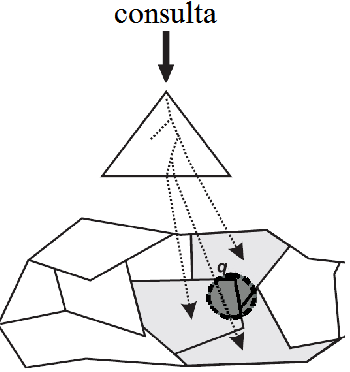
\includegraphics[width=0.32\columnwidth]{chapter2/candidate_regions.png}%\label{fig:slimbe:a}
    \label{fig:am_model}
    }
\subfigure[]
    {
    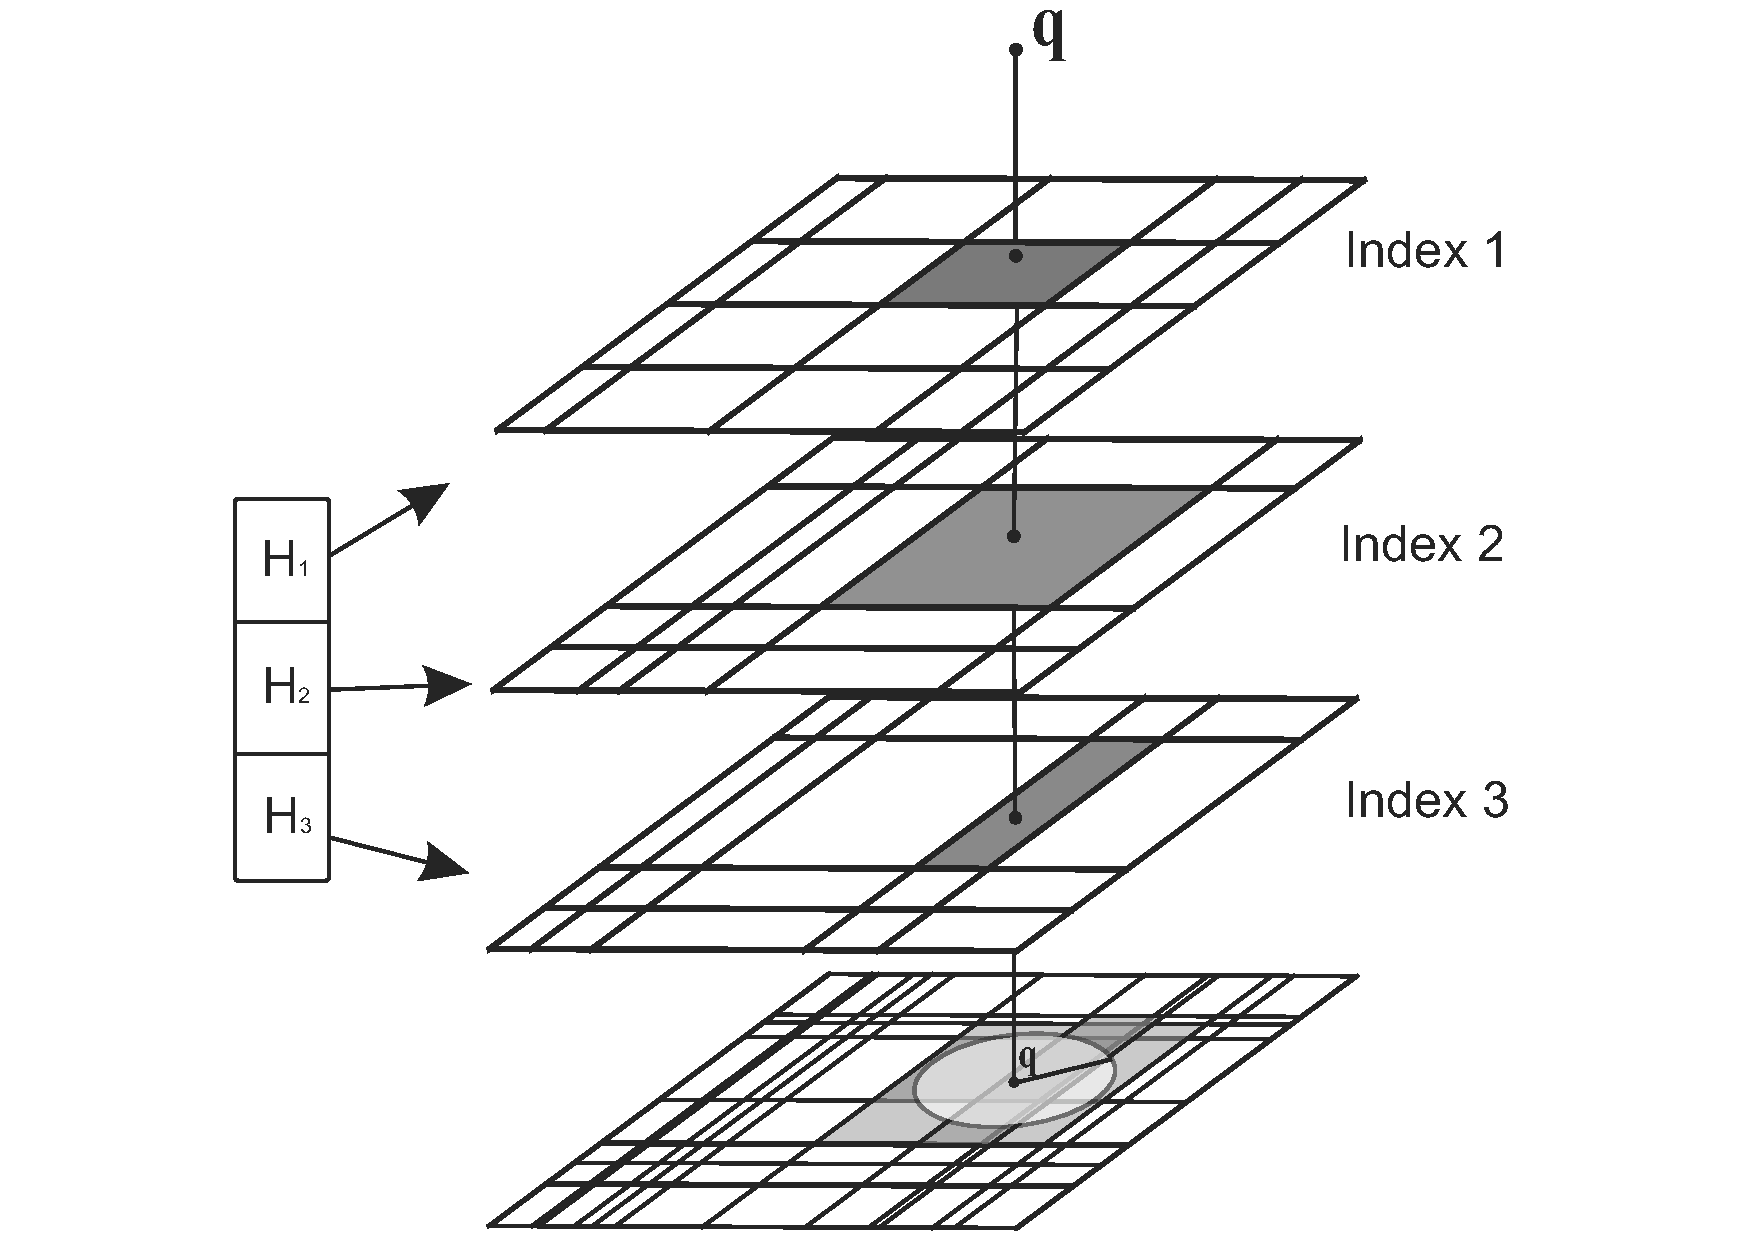
\includegraphics[width=0.37\columnwidth]{chapter2/lsh_basic_gray.pdf}%\label{fig:slimbe:a}
    \label{fig:lsh_model}
     }
\caption{Unificación del modelo de consulta por similitud. (a) Los Métodos de Acceso Métricos (MAMs). (b)  \textit{Locality Sensitive Hashing} (LSH).}
\label{fig:search_model}
\end{figure}


\section{Dominio de datos}

la concepción de un método de búsqueda debe considerar la naturaleza de los datos, a fin de explotar ciertas propiedades del espacio en donde están embebidos.

La gran mayoría de métodos de búsqueda supone que los datos pertenecen a un espacio n-dimensional. Esos espacios están en $R^n$, lo que permite el uso de propiedades geométricas en la solución. Por otro lado, algunos métodos tienen exigencias menos rigurosas, como el caso de los métodos basado en espacios métricos, que solo usan las distancias entre los puntos, y ninguna otra propiedad geométrica.


\subsection{Espacios Métricos}

Un espacio métrico es definido como  $\mathbb{M} = <S, d>$, donde $S$ es un universo de elementos y $d$ es una función de distancia (o métrica), definida sobre los elementos en $S$, que mide la disimilitud los objetos y satisfacen las siguientes condiciones, $\forall x, y, z \in S$:


\begin{tabular}{ l l }
  (1) $d(x, y) \geq 0   $ & positividad\\
  (2) $d(x, y) = 0 \leftrightarrow x = y$ & reflexibidad\\
  (3) $d(x, y) = d(y, x)$ & simetria\\
  (4) $d(x, y) \leq d(x, z) + d(y, z)$ & desigualdad triangular\\
\end{tabular}
\vspace{0.5cm}

La desigualdad triangular es considerado una de las propiedades mas importantes, pues es utilizada para establecer los límites del valor de distancia entre dos objetos sin la necesidad del cálculo real de distancia, acelerando así los algoritmos de consulta por similitud. Mas específicamente, dados los valores de distancia $d(x,z)$ y $d(y, z)$, los limites para el valor (desconocido) de $d(x, y)$ son $|d(x,z) - d(y, z)| \leq d(x, y) \leq d(x,z) + d(y, z)$.

No todas las propiedades (1)-(4) son necesarias para todos los métodos. Por ejemplo, se puede substituir (2) por una propiedad mas débil $\forall x \in S, d(x,x) = 0$, tornando el espacio pseudo-métrico. Los métodos que no obedecen las propiedades (3), (4) o ambas son típicamente llamados no métricos.


\subsection{Espacios Multidimensionales}

Si los objetos del dominio $S$ corresponden a los vectores de valores numéricos entonces el espacio es llamado Espacio Multidimensional o Espacio Vectorial con Dimensión Finita. Los objetos de un espacio multidimensional de dimensión $n$ (o $n$-dimensional) son representados por $n$ coordenadas de valores reales ${x_1, ..., x_n}$.

Las funciones de distancia métrica mas común para medir la similitud entre elementos en un Espacio Multidimensional son de la familia $L_p$, o Minkowski, definidas por:

\begin{equation}\label{lpnorm}
 L_p ((x_1,...,x_n), (y_1,...,y_n)) = (\sum_{i=1}^{n} |x_i - y_i|^p)^{1/p}
\end{equation}

\begin{itemize}

\item La distancia $L_1$ es también conocida como distancia \textbf{Manhattan}, y corresponde a una  simple suma de las diferencias absolutas de los componentes.

\item La distancia $L_2$ es también conocida como distancia \textbf{Euclidiana}, y corresponde a la idea usual de distancia en espacios $2D$ o $3D$.

\item La distancia $L_{\infty}$ es también conocida como \textbf{Chebychev}, y corresponde a la diferencia máxima absoluta entre los componentes, definida por:

\begin{equation}
   L_{\infty} ((x_1,...,x_n), (y_1,...,y_n)) = max_{i=1}^{n} |x_i - y_i|
\end{equation}

\end{itemize}

\begin{figure}[htp]
\centering
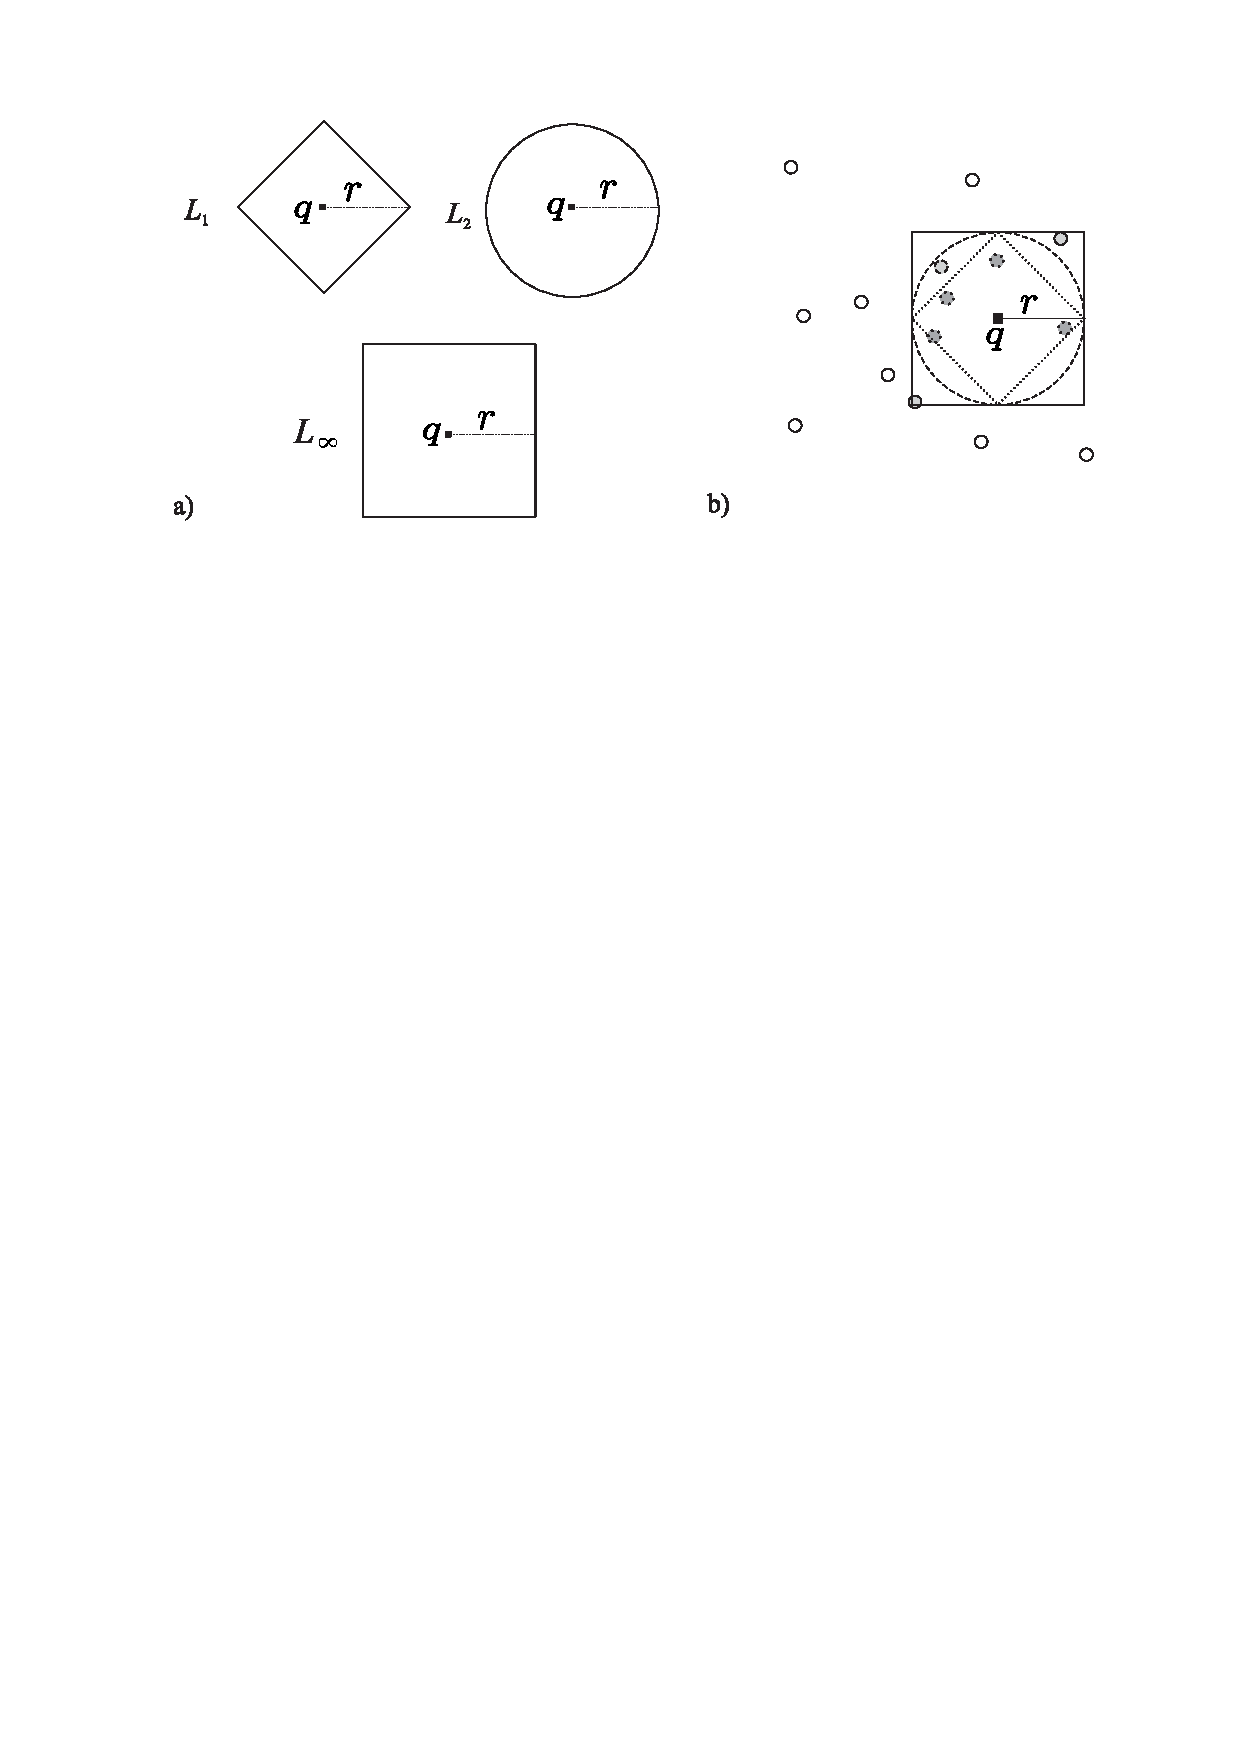
\includegraphics[width=0.9\columnwidth]{chapter2/lpnorms.pdf}
\caption{(a) Formas geométricas que ilustran la delimitación de una  región de búsqueda de acuerdo con la métrica $L_p$ utilizada. (b) Ejemplo de consulta por rango para diferentes métricas de la  familia $L_p$.}
\label{fig:lpnorms}
\end{figure}

La Figura \ref{fig:lpnorms}(a)  ilustra,  las distancias de la familia  $L_p$, el conjunto de puntos que están a la misma distancia $r$, a partir de un centro $q$, en un  espacio bi-dimensional.

La Figura \ref{fig:lpnorms}(b) representa un conjunto de objetos en un  espacio bi-dimensional, un objeto de consulta $q$, un radio de consulta $r$, los conjuntos de respuesta y tres métricas utilizadas: $L_1$, $L_2$ e $L_{\infty}$.

La \textbf{distancia de coseno} presentada en la Ecuación \ref{eq:2_3} es otra métrica de distancia popular para la búsqueda de $NN$ que ha demostrado ser particularmente eficaz para la recuperación de documentos \cite{Manning,Ravichandran}.

\begin{equation}\label{eq:2_3}
	    d_{cosine}(X_i,X_j) = 1 - \frac{\sum\nolimits_{k=1}^{D} x_{ik} x_{jk}}{\sqrt{\sum\nolimits_{k=1}^{D} x_{ik}^2}\sqrt{\sum\nolimits_{k=1}^{D} x_{jk}^2}}
\end{equation}

También encontraremos la \textbf{distancia de Hamming} ampliamente en esta tesis, ya que es la métrica por defecto para comparar cadenas binarias (Ecuación \ref{eq:2_4})

\begin{equation}\label{eq:2_4}
	   d_{hamming}(b_i,b_j) = \sum_{k=1}^{D} \delta[b_{ik} \neq b_{jk}]
\end{equation}

La función $\delta(.) = 1$ si su argumento es verdadero, y 0 en caso contrario. Por lo tanto, la distancia de Hamming cuenta el número de dimensiones correspondientes (bits) que no son iguales en los dos \textit{hashcodes}. \\

\section{Consultas por Similitud}\label{sec:consultas-similaridade}

Aplicaciones en la recuperación de información por similitud, por lo general crea un universo de objetos $\mathbb{U}$  y una función $d: \mathbb{U} \times \mathbb{U} \rightarrow \mathbf{R} $ que mide la distancia entre dos objetos en $\mathbb{U} $. En los espacios métricos, definimos $\mathbb{S} \subseteq \mathbb{U} $ como un conjunto finito de objetos, donde la función $d()$ mide la disimilitud entre objetos.

Dado un objeto de consulta $q \in \mathbb{U} $,  los objetos similares a $q$  se pueden recuperar de acuerdo a los siguientes tipos de consultas por similitud:

\paragraph{Consulta por radio (\textit{range query} Rq (q, r))} consulta que tiene como objetivo recuperar los objetos similares a $q$ que están dentro del rango de la consulta $r$.

\begin{equation}
    Rq(q, r) = \{ u \in S | d(u, q) \leq r \}
\end{equation}

En la Figura \ref{fig:rangeQuery} se representa una consulta por rango en un espacio bi-dimensional con la métrica $L_2$. Los elementos contenidos por el radio $e$ componen la respuesta. Vale recordad que no es necesario que el elemento de consulta pertenezca al conjunto de datos de búsqueda, debiendo este pertenecer al mismo dominio de datos.

\begin{figure}[htp]
\centering
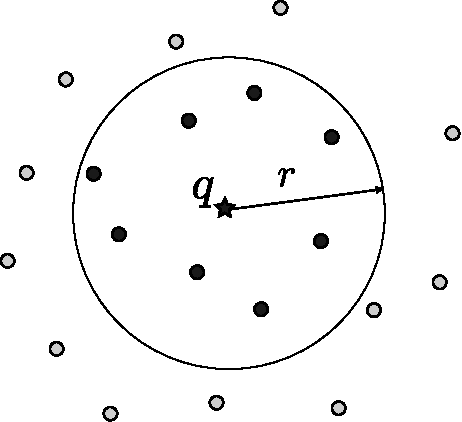
\includegraphics[width=0.3\columnwidth]{chapter2/range_query.pdf}
\caption{Ejemplo de consulta por rango.}
\label{fig:rangeQuery}
\end{figure}


\paragraph{Consulta de los k-vecinos más cercanos (\textit{k-Nearest neighbor query} - $kNN (q, k)$)} consulta que tiene como objetivo recuperar los $k$ objetos más cercanos al objeto de búsqueda $q$. O más formalmente, los $k$ vecinos más próximos definen el conjunto  $ C = \{s_1,s_2,...,s_k\} $ en que:

\begin{equation}
    \forall s_i \in C, \forall x_j \in S - C, d(q, s_i) \leq d(q, x_j)
\end{equation}

La Figura \ref{fig:knnQuery} ejemplifica una consulta kNN en un espacio bi-dimensional con la métrica $L_2$. En la figura, la consulta tiene como entrada el elemento de consulta $q$ y el valor de $k$ igual a $3$.  Los elementos conectados a $q$ corresponden al consulto de respuesta, considerando que en el ejemplo el elemento $q$ no pertenece al conjunto de datos.

\begin{figure}[htp]
\centering
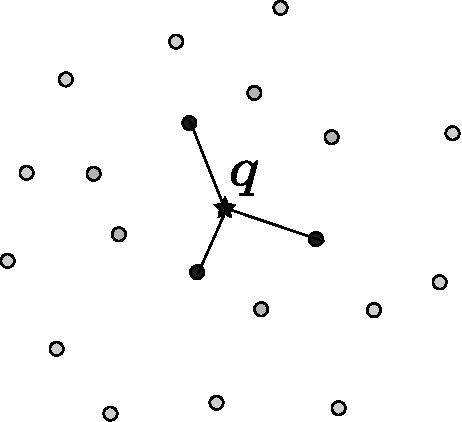
\includegraphics[width=0.28\columnwidth]{chapter2/knn_query.pdf}
\caption{Ejemplo  de consulta de los k-vecinos más cercanos.}
\label{fig:knnQuery}
\end{figure}
 

\paragraph{Consulta por rango aproximada - $(1 + \varepsilon)  Rq(q, r)$}

Consulta que busca recuperar los objetos cercanos a $q$ que se encuentran dentro del radio de consulta  $(1 + \varepsilon) \times r$. O, más formalmente:

\begin{equation}
    (1 + \varepsilon) Rq(q, r) = \{ u \in S | d(u, q) \leq (1 + \varepsilon) \times r \}
\end{equation}

La Figura \ref{fig:AproximateRangeQuery} ejemplifica una consulta de este tipo para $L_2$. Los elementos dentro del radio de consulta  $(1 + \varepsilon)\times r$ componen la respuesta aproximada.
\begin{figure}[htp]
\centering
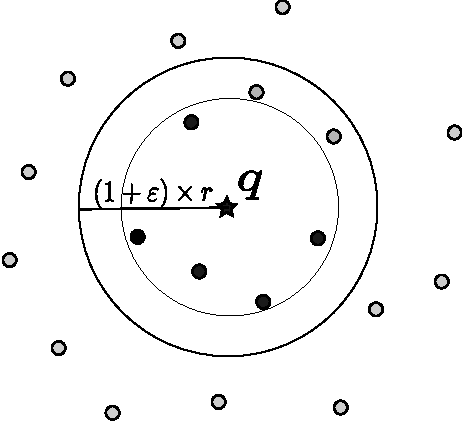
\includegraphics[width=0.32\columnwidth]{chapter2/app-range_query.pdf}
\caption{Ejemplo de consulta  por  rango aproximada.}
\label{fig:AproximateRangeQuery}
\end{figure}
%@ refazer figura


\paragraph{Consulta Aproximada a los $k$-vecinos más cercanos  - $(1 + \varepsilon) - kNN(q, k)$}
Sea $r$ la distancia entre el objeto de consulta $q$ y el elemento más distante entre los $k$ verdaderos vecinos más próximos, esto es,

\begin{equation}
r = max\{ s_j \in S | d(q, s_j)\}
\end{equation}

La búsqueda $(1 + \varepsilon)-kNN$  para los $k$ elementos  mas similares a $q$ consiste en encontrar un conjunto $C' = \{s_1', s_2', ..., s_k'\}$ en donde,

\begin{equation}
\forall s_i' \in C', d(q, s_i') \leq (1 + \varepsilon) \times r
\end{equation}

El factor $(1 + \varepsilon)$  es usualmente llamado  \textbf{factor de aproximación}, y indica que el conjunto de la solución $C'$ está dentro de un \textbf{error relativo}  $\varepsilon$  a la respuesta exacta.  Ver Figura \ref{fig:nearbyKnnQuery}.
\begin{figure}[htp]
\centering
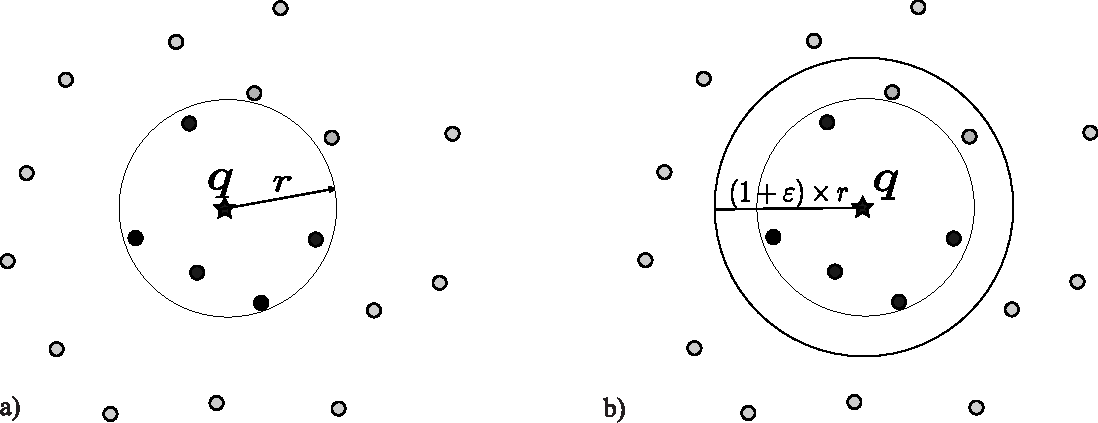
\includegraphics[width=0.85\columnwidth]{chapter2/nearby_knn_query.pdf}
\caption{Búsqueda aproximada 5-NN. (a) busca exacta. (b) busca aproximada.  }
\label{fig:nearbyKnnQuery}
\end{figure}

 

\section{La Maldición  de la alta Dimensionalidad} \label{sec:madicao-dimensionalidade}

La eficiencia de los métodos de búsqueda por similitud dependen mucho de la dimensionalidad. Aunque el tiempo de búsqueda pueda alcanzar un costo logarítmico en relación al tamaño de los datos, este va crecer exponencialmente con la dimensionalidad de los datos.

Para dimensiones moderadas, la mayoría de los métodos ejecutas las consultas de manera suficientemente eficientes para permitir una solución exacta  en un tiempo razonable. Para dimensiones más altas, se vuelve viable el uso de métodos aproximados,  lo que implica en un \textit{trade-off}  entre la precisión y la eficiencia. Para dimensiones más altas ese \textit{trade-off}  va convertirse progresivamente más relevante, resultando en penalidades mayores en términos de precisión, a fin de obtener una eficiencia aceptable.

El problemas de ``la maldición de la alta dimensionalidad'' fue estudiado originalmente por Bellman \cite{citeulike:Bellman}, observando que particiones del espacio de soluciones en problemas de optimización son ineficientes en problema con datos en altas dimensiones. Los efectos de ``maldición'' en Métodos de Acceso Espaciales (MAEs) y Métodos de Acceso Métricos (MAMs) son discutidos en  \cite{aleman_high_dimensional, WhatsWrong, DBLP:journals/corr/abs-0906-0391}.

%\section{Soluciones Aproximadas}\label{sec:solucoes-aproximadas}
\section{Búsqueda aproximada  de los vecinos más cercanos (ANN)}

En esta sección   definimos formalmente el problema de la búsqueda del vecino más cercano (Nearest Neighbor search - NN). Se examinará entonces la versión simplificada de la búsqueda NN conocida como búsqueda NN aproximada, el campo en el que se basa esta tesis, y describirá cómo difiere de los algoritmos alternativos para resolver el problema de búsqueda NN.

Los trabajos descritos en este capitulo todos comparten la definición del mismo problema. Dado un conjunto de datos X que consiste de N puntos ($X \in R ^ {NxD} = [x_1, x_2,..., x_N]^T$), donde cada punto $x_i \in R^D$ es un vector D-dimensional de valores reales (vector característica). El objetivo es construir un conjunto de $m$ funciones hash $\{ h_m : R^D \rightarrow {0, 1}\}_{m=1}^K$ cuya salida puede ser concatenada como [$h_1(x_i), h_2(x_i), ..., h_\Nhashfunctions(x_i)$]  el cual cumple la función de codificar el vector característica.  Para codificar se necesitan funciones \textit{hash} que preserven la similitud del espacio original.  
 
La búsqueda de vecinos más cercanos se puede definir como el problema de recuperar el punto de datos más cercano $ NN(q) $ para una consulta $ q \in R^D$ en un conjunto de datos de $N$ puntos  $ [x_1. x_2 , ..., x_N]^T $ donde $x_i \in R^D$. La similitud entre los puntos   se define por una función de distancia  $\{ d(.,.) : R^D \times R^D  \}$.   Es fácil generalizar esta definición de problema para devolver los vecinos $K$ más cercanos a la consulta. Esta variante se conoce   como búsqueda k-NN y es un componente fundamental en una amplia gama de diferentes métodos de aprendizaje de máquinas. La función de distancia $d(x,y)$ entre los puntos de datos se suele calcular utilizando una métrica de distancia genérica como la $l_p - norm$ (Ecuación \ref{lpnorm}).

Para buscar $NNs$ a una consulta necesitamos construir una estructura de datos o algoritmo que tome nuestra noción seleccionada de distancia y recupera los puntos de datos que están cerca de la consulta bajo esa métrica de distancia específica. La búsqueda por fuerza bruta es un algoritmo sencillo para resolver el problema de búsqueda del vecino más cercano con cualquier métrica de distancia deseada. En la búsqueda por fuerza bruta se calcula la distancia a todos los puntos en la base de datos y los puntos  con la menor distancia a la consulta son devueltos como el vecino más cercano. Las ventajas de la búsqueda de la fuerza bruta son su simplicidad de la puesta en práctica y su garantía que los vecinos más cercanos   serán recuperados eventualmente. Sin embargo, comparar exhaustivamente la consulta con cada punto en la base de datos da una complejidad temporal $O (ND)$ que hace rápidamente la búsqueda de fuerza bruta intratable para la búsqueda de vecinos más cercanos a través de conjuntos de datos con muchos puntos de datos (N) y una dimensionalidad moderada a alta (RE). En esta situación, se requiere un enfoque más informado del problema de búsqueda del vecino más cercano.\\
 
En la  sección \ref{sec:lsh}, introduciremos el método \textit{Locality Sensitive Hashing (LSH)}, una familiar de algoritmos que proveen un método para resolver búsqueda aproximada de los vecinos mas próximos con un tiempo de consulta constante. 

\subsection{\textit{Locality Sensitive Hashing}}\label{sec:lsh}

Algunos trabajos de búsqueda aproximada  \cite{lsh_hamming,Datar2004,hashing_algoritghms_survey} exploran la idea de mapear los objetos de un conjunto de datos y agruparlos en  \textit{buckets} con el objetivo de ejecutar consultas por similitud aproximada dentro de los  \textit{buckets} asociados al objeto de consulta. En particular, el método \textit{Locality Sensitive Hashing} (LSH) fue ideado para resolver eficientemente consultas por rango aproximada $((1+\epsilon) Rq(q, r))$. Como fue definido en la Sección  \ref{sec:consultas-similaridade}, este tipo de consulta busca recuperar los objetos que se encuentran dentro de un radio de consulta $(1+\epsilon) \times r$. La idea principal es que, si dos objetos son próximos en el espacio original, esos dos objetos tienden a permanecer próximos después de una operación de proyección escalar randomica. Así, dada una función \textit{hash} $h(x)$ que mapea un objeto ($x$) de dimensión $n$ a un valor unidimensional, la función es sensible a la localidad si la posibilidad de mapeamiento de dos objetos $x_1$, $x_2$ al mismo valor crece a la medida que la distancia  $d(x_1, x_2)$  disminuye. Formalmente:

\paragraph{Definición} Dado un valor de distancia $r$, un factor de aproximación $1+\epsilon$, las probabilidades $P_1$ y $P_2$, tal que $P_1 > P_2$, la función \textit{hash}  $h()$ es sensible a la localidad de los datos si satisface las siguientes condiciones:

\begin{itemize}
\item $Se \ d(x_1, x_2) \leq r \Rightarrow Pr[h(x_1) = h(x_2)]  \geq P_1$.

Esto quiere decir que para dos objetos  $x_1$ y $x_2$ en $R^n$  que están lo suficientemente próximos,  hay una probabilidad   $P_1$ que ellos caigan en el mismo \textit{bucket}.

\item $Se\ d(x_1, x_2) > (1+\epsilon) \times r  \Rightarrow Pr[h(x_1) = h(x_2)] \leq P_2$.

Esto quiere decir que para dos objetos $x_1$ y $x_2$ en $R^n$ que están distantes, hay una probabilidad $P_2 < P_1$ que ellos caigan en el mismo  \textit{bucket}.

\end{itemize}

El esquema propuesto en \cite{Datar2004} fue proyectado para trabajar con distribuciones p-estables de la siguiente manera: calcular el producto escalar $\vec{a} \cdot \vec{x}$ para atribuir un valor \textit{hash} para cada vector $x$. La función  \textit{hash} precisa de valores randomicos $\vec{a}$ y $b$, en que $\vec{a}$ es un vector n-dimensional con valores independientemente escogidos a partir de distribuciones p-estables (Cauchy o Gaussiana) y $b$ es un número real escogido dentro de un intervalo $[0,\omega]$. Por tanto la función \textit{hash} $h(x)$ esta dada por:


\begin{equation}\label{eq:lsh}
    h(x) = \lfloor\frac{\vec{a} \cdot \vec{x} + b}{ \omega }\rfloor
\end{equation}

La ecuación \ref{eq:lsh} tiene una interpretación simple. Considere la Figura \ref{fig:quantization}: $\vec{p_1}$ y $\vec{p_2}$ son dos vectores en $\mathbf{R}^2$, $\vec{a}$ es un vector normal unitario e $b$ es un número randomico real. A inclinación de la recta pasando por el origen coincide con la dirección de $\vec{a}$. Así, $\vec{p_1}$  es proyectado sobre la línea $\vec{a}$  calculando el producto escalar  $\vec{a} \cdot \vec{p_1}$. Esa proyección es cuantizada en intervalos de tamaño fijo  $\omega$, definiendo el punto A. El mismo procedimiento es repetido para $\vec{p_2}$, definido el punto B.

\begin{figure}[htp]\centering
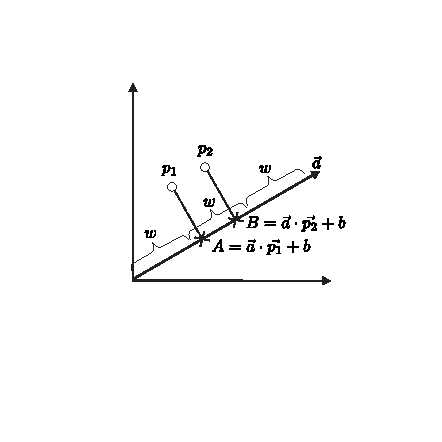
\includegraphics[width=0.3\columnwidth]{chapter2/lsh_projection.pdf}
\caption{Interpretación geométrica de proyección de los  vectores $\vec{p_1}$ y $\vec{p_2}$ en LSH.}
\label{fig:quantization}
\end{figure}

Para amplia a diferencia entra las probabilidades $P_1$ y $P_2$ se puede usar $\Nhashfunctions$ funciones \textit{hash} diferentes. Esto aumenta las probabilidades dado que \mbox{$(P_1/P_2)^\Nhashfunctions > P_1/P_2$}, asegurando así que si dos objetos están muy distantes, la probabilidad de que caigan en el mismo \textit{bucket} sea baja. Sin embargo, aunque sea importante evitar que objetos distantes caigan en el mismo \textit{bucket} para preservar la proximidad espacial, esto no es una condición suficiente. Es igualmente importante asegurar que objetos próximos en el espacio original tengan una alta probabilidad que aparecer en el mismo \textit{bucket}. Así, como eso no puede ser alcanzado usando solo una estructura \textit{hash}, LSH resuelve ese problema considerando $L$ proyecciones independientes, ósea, la construcción de $L$ tablas \textit{hash} ($L$ subíndices) \cite{lshtutorial,taoLSBLSH}.

Así usando colecciones diferentes de $\Nhashfunctions$ funciones \textit{hash} $H = \{h_1, h_2, ..., h_\Nhashfunctions\}$, siendo una colección cada sub-indice, cada objeto $x$ de un conjunto de datos es mapeado en \textit{buckets}, efectivamente particionando el conjunto de datos en varios grupos pequeños (los \textit{buckets}) para cada uno de los $L$ subindices. La estructura de datos será entonces formada por $L$ subíndices. LSH divide el espacio de búsqueda empleando $\Nhashfunctions$ funciones \textit{hash} escogidas aleatoriamente de una distribución Gaussiana (o Cauchy). Un número de funciones \textit{hash} $\Nhashfunctions$ determina cuan esparzo o denso será el espacio de búsqueda. Al aumentar el valor de $\Nhashfunctions$, los objetos tiendes a ser distribuidos en \textit{buckets} de manera bastante uniforme, reduciendo la precisión de las consultas ya que es más probable que objetos similares caigan en \textit{buckets} diferentes. Para atenuar ese efecto negativo, son necesarias muchas tablas \textit{hash}. Por otro lado, al disminuir el valor de $\Nhashfunctions$, el número de colisiones aumenta, así como el número de elemento a ser tratados en tiempo de consulta. Así, el desempeño de las consultas disminuye.


El proceso de indexación de un conjunto de datos $S$ usando LSH es mostrado en el Algoritmo \ref{alg:lshalgorithm}. Cada elemento $x$ del conjunto de elementos $S$ es proyectado usando   $\Nhashfunctions$  funciones \textit{hash} que transforma el elemeno $x$ en $\Nhashfunctions$  números reales ($x'$, el vector \textit{hash}). Esos $\Nhashfunctions$  números son entonces cuantificados con un único número ($g$).

\begin{lstlisting}[mathescape, frame=single, label=alg:lshalgorithm,caption=Algoritmo de construcción para LSH]
Entrada: El conjunto de dados  $S$
Salida: Todos los objetos mapeados en las $L$ tablas $hash$
  for $i = 1$ to $L$ do
    $H_{i} \Leftarrow \{h_1,...,h_\Nhashfunctions\}$       //Inicializar tabla $T_i$ con un conjunto de funciones $hash$ $H_i$
  end for
  for $i = 1$ to $L$  do
    foreach $x$ en $S$ do
      $x' \Leftarrow $ $<h_1(x),...,h_\Nhashfunctions(x) >$  //Proyectar $x$:  $\Nhashfunctions$ veces usando el conjunto de funciones $hash$ $H_{i}$
      $g \Leftarrow quantize(x')$                            // Calcular el valor $hash$ final
      $I \Leftarrow T_i[\  g $ mod $ | T_{i} |\ ]$     //localizar el $bucket$ $I$
      Insertar la entrada $<x, g>$  en $I$, almacenando la referencia de $x$ y el valor $g$
    end for
  end for
\end{lstlisting}


Una vez que cada \textit{bucket} es definido en términos de similitud (esto es, elementos semejantes tienden a ser encontrados en el mismo \textit{bucket}, es probable encontrar los vecinos más próximos a un objeto $q$ en los \textit{buckets} recuperados por cada conjunto de funciones \textit{hash}). Así, en vez de hacer comparaciones para reducir el espacio de búsqueda, LSH mapea directamente los objetos a los \textit{buckets}. Luego, es posible obtener un costo sub-linear en las consultas. En una consulta kNN, a fin de retornar los $k$ vecinos más próximos, apenas las distancias entre $q$ y los elementos dentro de los \textit{buckets} son calculados. En una consulta por rango sucede lo mismo, mas la condición de consulta es diferente y solo los elementos dentro del radio de consulta son retornados. El algoritmo de consulta por rango aproximada es descrito en el Algoritmo  \ref{alg:lsh_rq}.

\begin{lstlisting}[mathescape, frame=single, label=alg:lsh_rq,caption=Consulta por rango aproximada usando LSH]
Entrada: El objeto de consulta $q$ y el radio de consulta $r$
Salida:  Los objetos que satisfacen las condiciones de consulta.
  for $i = 1$ to $L$  do
    $q' \Leftarrow $ $<h_1(q),...,h_\Nhashfunctions(q)>$ //Proyectar $x$:  $\Nhashfunctions$ veces usando el conjunto de funciones hash $H_{i}$
    $g \Leftarrow quantize(q')$   //  calcular el valor hash final
    $I \Leftarrow T_{i}[\  g $ mod $ | T_{i} |\ ]$   //localizar el bucket $I$
    foreach $e$ en $I$ do
      if $e.g = g  \wedge  d(q, e.x) \leq r $ then
        retornar $e.x$ si no fue reportado
      end if
    end for
  end for
\end{lstlisting}

El algoritmo kNN puede ser obtenido por medio de simples modificaciones en el Algoritmo \ref{alg:lsh_rq}. Básicamente, el algoritmo kNN terminará cuando se encuentre $k$ objetos distintos o si no hubiere más \textit{buckets} para explorar. No obstante, es importante recordar que LSH garantiza resultados de calidad previsible apenas para consultas por rango aproximada $((1+\epsilon)-Rq(q, r))$. Además, algunos inconvenientes de LSH no fueron resueltos por completo, por ejemplo: (1) LSH requiere varios sub índices de moco que cada subíndice organiza el conjunto de datos entero usando una tabla \textit{hash} con funciones \textit{hash} independientes. Esa exigencia es extremadamente crítica para mejorar la precisión de búsqueda, mas lleva a un alto consumo de memoria; (2) LSH tiene una dependencia crítica de los parámetros de dominio, que determina el número de funciones \textit{hash} y el número de tablas \textit{hash}.


 En \textit{hash} los autores propusieron LSH Multi-probe, que busca mantener un costo de memoria aceptable. LSH Multi-prove está basado en el LSH clásico, mas en cuanto el algoritmo de consulta LSH examina apenas un \textit{bucket} para cada tabla \textit{hash}, LSH Muli-probe examina los \textit{buckets} que son susceptibles de contener los resultados de consulta por cada tabla \textit{hash}. Consecuentemente, el número de tablas \textit{hash} es reducido sin perdida significativa de precisión. Intuitivamente esta propuesta verifica los \textit{buckets} de forma más inteligente, generando $\tau$ $probes$ por cada tabla   \textit{hash}, lo que permite explorar $\tau$ \textit{buckets} por sub-índice, y como consecuencia, aumentar el número de candidatos sin incrementar el número de subíndices.

Una investigación más reciente sobre el método LSH \cite{modelinglsh}  muestra que el desempeño en las consultas no solo dependen de la distribución general del conjunto de datos, mas también de la distribución local en torno a un objeto de consulta. En el método LSH Multi-probe, un número fijo de $probes$ puede ser insuficiente para algunas consultas y mayor del que es necesario para otras. No obstante aun es complicado ajustar el número de funciones \textit{hash} asociado al radio de consulta.

Dado que los parámetros también dependen del número de objetos a ser indexados, el método LSH no es una solución incremental. Para lidiar con este problema, una nueva propuesta fui presentado, el método LSH-Forest \cite{lshforest}. Esa técnica fue desarrollada para soportar auto-ajuste en relación al número de funciones \textit{hash}. Esencialmente, el método LSH-Forest es una colección de arboles de prefijos donde cada una puede tener un número diferente de funciones \textit{hash}. No obstante, aun es necesario ajustar el número de subíndices, o sea, el número de arboles prefijo. Además, no esta claro su desempeño en sistemas que trabajan con datos distorsionados, en donde se tiende a verificar más candidatos del que es necesario en pequeñas áreas densas y tener candidatos insuficientes para los puntos de consulta en áreas esparzas.


En ese mismo escenario,  la técnica LSH Multi-level \cite{DBLP:journals/jidm/OcsaS10}, desarrollada en el contexto de este trabajo, propone un nuevo esquema de \textit{hashing} para resolver algunos de esos problemas. Especificamente, utilizan un esquema multiresolución para resolver la dependencia de parámetros de dominio. El método no espera los parámetros del dominio de datos, pues, se adapta dinámicamente durante el proceso de indexación, gracias a las habilidades auto-adaptativas de la estructura del índice multi-nivel. Este método presenta un mejor desempeño en termino de tiempo y espacio comparado con otras propuestas \textit{hash}, pues la técnica multi-nivel distribuir los objeto en \textit{buckets} de manera uniforme en todos los niveles. Esto porque, en contraste con LSH, el método LSH Multi-level usa la estructura multi-resolución para calcular y localizar los vectores \textit{hash} apropiados para una consulta especifica. Así, varios vectores \textit{hash} de diferentes resoluciones son calculados por cada índice en el proceso de consulta y, como consecuencia, no se precisa de mas índices para garantizar resultados de la misma calidad.

Recientemente, en \cite{taoLSBLSH}  los autores propusieron el método LSB-Forest. Este trabajo mejor la técnica LSH-Forest, y a fin de garantizar la calidad y eficiencia de recuperación de datos multidimensionales, utiliza representaciones basadas en \textit{space-filling curves} y arboles B. De ese modo, los valores \textit{hash} son representado como valores unidimensionales usando tanto la proyección LSH como las curvas Z. Además, varios arboles B son usados para indexas los datos con el objetivo de mejorar la calidad de los resultados. Una desventaja de los arboles LSB es que usa lecturas/escrituras randomicas, lo que conlleva requiere un número considerable de accesos a disco cuando el conjunto de datos es grande. Para resolver ese problema, el método HashFile \cite{lshHashFile}  fue propuesto. Como será detallado en la siguiente sección, en comparación a los métodos actuales LSH, el método HashFile solo divide recursivamente los \textit{buckets} densos para alcanzar particiones mas equilibradas. Cada \textit{bucket} almacena un número fijo de objetos, mas el método aprovecha la lectura secuencial en vez de usar el acceso randomico, como es el caso en los arboles  B. Este método esta basado en conceptos de proyección aleatoria (\textit{Random Projection}).
 
 

\subsection{LSH con Projección Aleatória}\label{sec:hashfile}

%In this dissertation I will be primarily interested in the locality sensitive hash function
%family for the inner product similarity which traditionally has been used as a baseline
%for comparison by existing research in the learning to hash literature. The inner product
%similarity is defined in Equation 2.6.


%LSH puede ser usado también con familia de funciones \textit{hash} para buscar la similitud usando producto punto el cual ha sido tradicionalmente usado como base de comparación en varias investigaciones. El producto punto es definido como:  

%\begin{equation}\label{eq:dotproduct}
%d(p, q) =   \Sigma_{i=1}^d h_i \cdot o_i \\
%                =  p^T q
%\end{equation}

%La ecuación \ref{eq:dotproduct} puede ser interpretado como la medida de similitud coseno entre dos vector unitarios   normalizados. La medida de similitud  coseno mide la cercanía entre dos puntos que están en un ángulo $\tetha$.
El algoritmo de proyección aleatoria (Random Projection) básicamente usa vectores aleatorios provenientes de una distribución estable. El algoritmo es robusto contra el ruido y utiliza un enfoque probabilístico, consiguiendo reducir significativamente el costo computacional de la búsqueda con una pequeña perdida de precisión. La naturaleza aleatoria de la técnica permite una comparación eficiente de secuencias muy largas para el descubrimiento de características relevantes.

Un caso de esta familia de funciones que usan protección aleatoria  es  el  método HashFile \cite{lshHashFile}  fue propuesto para responder consultas kNN exactas en el espacio $L_1$  y $L_2$. El método combina las ventajas de la proyección aleatoria  y la  lectura secuencial. 

%Al contrario de otros métodos basado en LSH, en donde cada  \textit{bucket} es asociado a una concatenación de $m$ valores \textit{hash}, este método particiona recursivamente  los \textit{buckets}  densos que son organizados en un estructura jerárquica. Note que al contrario de  la mayoría  de los métodos LSH, este método solo necesita de un sub-indice para garantizar resultados de calidad. De ese modo, dado un objeto de consulta $q$, el algoritmo de búsqueda solo explorar los \textit{buckets} que están cerca al objeto de consulta usando el esquema de búsqueda $\textit{top-down}$. Los \textit{top-down}. Los\textit{buckets}   candidatos en cada nodo son almacenados secuencialmente  en orden creciente  a su valor \textit{hash}  y  pueden ser eficientemente  cargados a memoria principal. Los resultados muestran que este método supera métodos recientes, que representan el estado del arte en métodos de indexación, para consultas kNN exactas y aproximadas.

\subsubsection{Projección Aleatória}

La proyección aleatoria es un método de reducción de la dimensionalidad de los datos que es computacionalmente eficiente y suficientemente preciso. Dado un conjunto de datos $S$ con $N$ puntos de dimensión $n$ y una matriz aleatoria  $ R_{n \times k} $, la proyección es calculada de la siguiente manera.

\begin{equation}
S'_{N \times k} = S_{N \times n} \times R _{n \times k}
\end{equation}

La proyección resulta en un conjunto de datos  $S'$ k-dimensional con $N$ puntos. La proyección aleatoria puede preservar la distancia $L_1$ o $L_2$ en un espacio reducido, lo que es especificado por el Lema Jonhson-Lindenstrauss.


\paragraph*{Lema de Jonhson-Lindenstrauss:} Dado $\epsilon > 0$ es un numero  $N$, sea $k$ un  entero positivo tal que $k \geq k_0 = O (\epsilon^{-2}log N)$. Para cada conjunto $S$ de $N$ puntos en  $\mathbb{R}^n$, existe $f: \mathbb{R}^n \rightarrow  \mathbb{R}^k$   tal que para todo $u,v \in S$, se tiene:

\begin{equation}\label{eq:JL-lemma}
  (1 - \epsilon) \parallel u - v \parallel^2 \leq \parallel f(u) - f(v) \parallel^2 \leq (1 + \epsilon)\parallel u - v \parallel^2
\end{equation}

%En los últimos años, el Lema de Jonhson-Lindenstrauss (JL) ha sido útil en la resolución de una variedad de problemas. La idea es la siguiente: al obtener una baja representación dimensional de los datos, JL acelera cierto algoritmo de forma significativa, en especial los algoritmos cuyo tiempo de ejecución dependen exponencialmente de la dimensión del espacio de trabajo (hay una serie de problemas prácticos para los cuales los algoritmos más conocidos tienen ese comportamiento). Al mismo tiempo, JL provee una garantía de conservación de la proximidad después de una operación de proyección sobre cada par de distancias y generalmente es suficiente para establecer que la solución encontrada en el espacio reducido es una buena aproximación de la solución óptima en el espacio original.

Algunos ejemplos de aplicación fueron presentado en \cite{Indyk:1998:ANN:276698.276876}. Por ejemplo, Indyk y Motwani mostraron que el Lema JL es útil para resolver el problema de búsqueda aproximada al vecino más cercano, donde después de algunos procedimiento de pre-procesamiento del conjunto de datos, consultas de este tipo son respondidas: Dado un punto arbitrario $x$ y un punto $y \in P$, para cada punto $z \in P$ se satisface $ \|x - z\| \geq (1 - \epsilon)\|x - y\|$.

\subsubsection{Restricción de la distancia para consultas kNN usando $L_1$}

Supongo que  $\mathcal{H}$  es una función \textit{hash}  derivada de  $R_{n \times k}$   tal que esta mapea un objeto $o$
 de dimensión $n$ en un valor unidimensional.

\begin{equation}\label{eq:hashfile}
\mathcal{H}(o) = \lfloor \Sigma_{i=1}^n h_i \cdot o_i \rfloor
\end{equation}

Dado que cada elemento $h_i$  está dentro de $\mathcal{H}$  para valores randomicos $\{-1,0,1\}$,  se puede   fácilmente  alcanzar un \textit{lower bound} para consultas con la  distancia $L_1$.

\paragraph*{Limite Inferior para $L_1$} Dado dos puntos $x$ y $y$ de dimensión $n$, y una función  \textit{hash} $\mathcal{H} : \mathbb{R}^n \rightarrow \mathbb{R}^1$ con  $h_i \in \{-1,0,1\}$, se tiene.

\begin{equation}\label{eq:LBL1}
 \parallel x - y \parallel_{L_1} \geq | \mathcal{H}(x) - \mathcal{H}(y) | - 1
\end{equation}

Así, una proyección aleatoria puede ser usada para particionar un gran volumen de datos en \textit{buckets}, en un espacio unidimensional. Las páginas en disco pueden ser almacenados secuencialmente en orden creciente al valor \textit{hash}. Así, dado un punto de consulta $q$ y la distancia $\lambda$ al vecino más próximo ya encontrados, si el valor \textit{hash} de $q$ y $h_q$, entonces de acuerdo con la relación presentada en la Ecuación \ref{eq:LBL1}, solo las páginas con valor \textit{hash} entre $[ h_q - \lambda, h_q + \lambda]$ necesitan ser accesadas. Los demás puntos fuera del intervalo pueden ser seguramente podados.

 

\subsubsection{Construcción del índice}

El método HashFile es construido siguiendo el esquema \textit{top-down}. Inicialmente, una función  \textit{hash}  es generada en el nodo raíz y se crea un archivo en disco para almacenar los datos. Dado que no es posible predecir la gama de valore  \textit{hash} , no se puede atribuir una colección de páginas de tamaño fijo con antecedencia. Así, apenas una página es reservada con un intervalo $(\infty,\infty)$. El tamaño de la página es fijo $B$, indicando que ella puede acomodar hasta $B$ puntos. Los primero $B$  objetos pueden ser insertados con éxito en esa página. Ahora, un nuevo objeto puede ser insertado en base a su valor \textit{hash}. Como nuevos objetos son insertados de forma continua, una operación de división ocurre y esos intervalos \textit{hash} se hacen menores. Finalmente, un objeto puede ser mapeado para un \textit{bucket} lleno donde los puntos tienen un mismo valor \textit{hash} y por tanto no puede ser dividido. Para insertar un nuevo objeto, se crea un nodo hijo con una nueva función \textit{hash}. Los puntos en esa página son extraído y son re-mapeados junto con un nuevo objeto en el nodo hijo.

La Figura   \ref{fig:HashFile_structure} ilustra un ejemplo de la estructura del árbol del método HashFile, así como la estructura lógica de un nodo interno del árbol. El árbol es construido por la inserción continua de los datos. Cuando un \textit{bucket} en el nodo padre no puede ser divido más, nodos hijos son creado para particionar el \textit{bucket} más denso. Por tanto, cada nodo interno contiene una lista de nodos hijos, como es ilustrado en la figura del ejemplo. Cada bloque representa una página con un intervalo \textit{hash}  $[l_i, h_i]$.

\begin{figure}[h]
\centering
 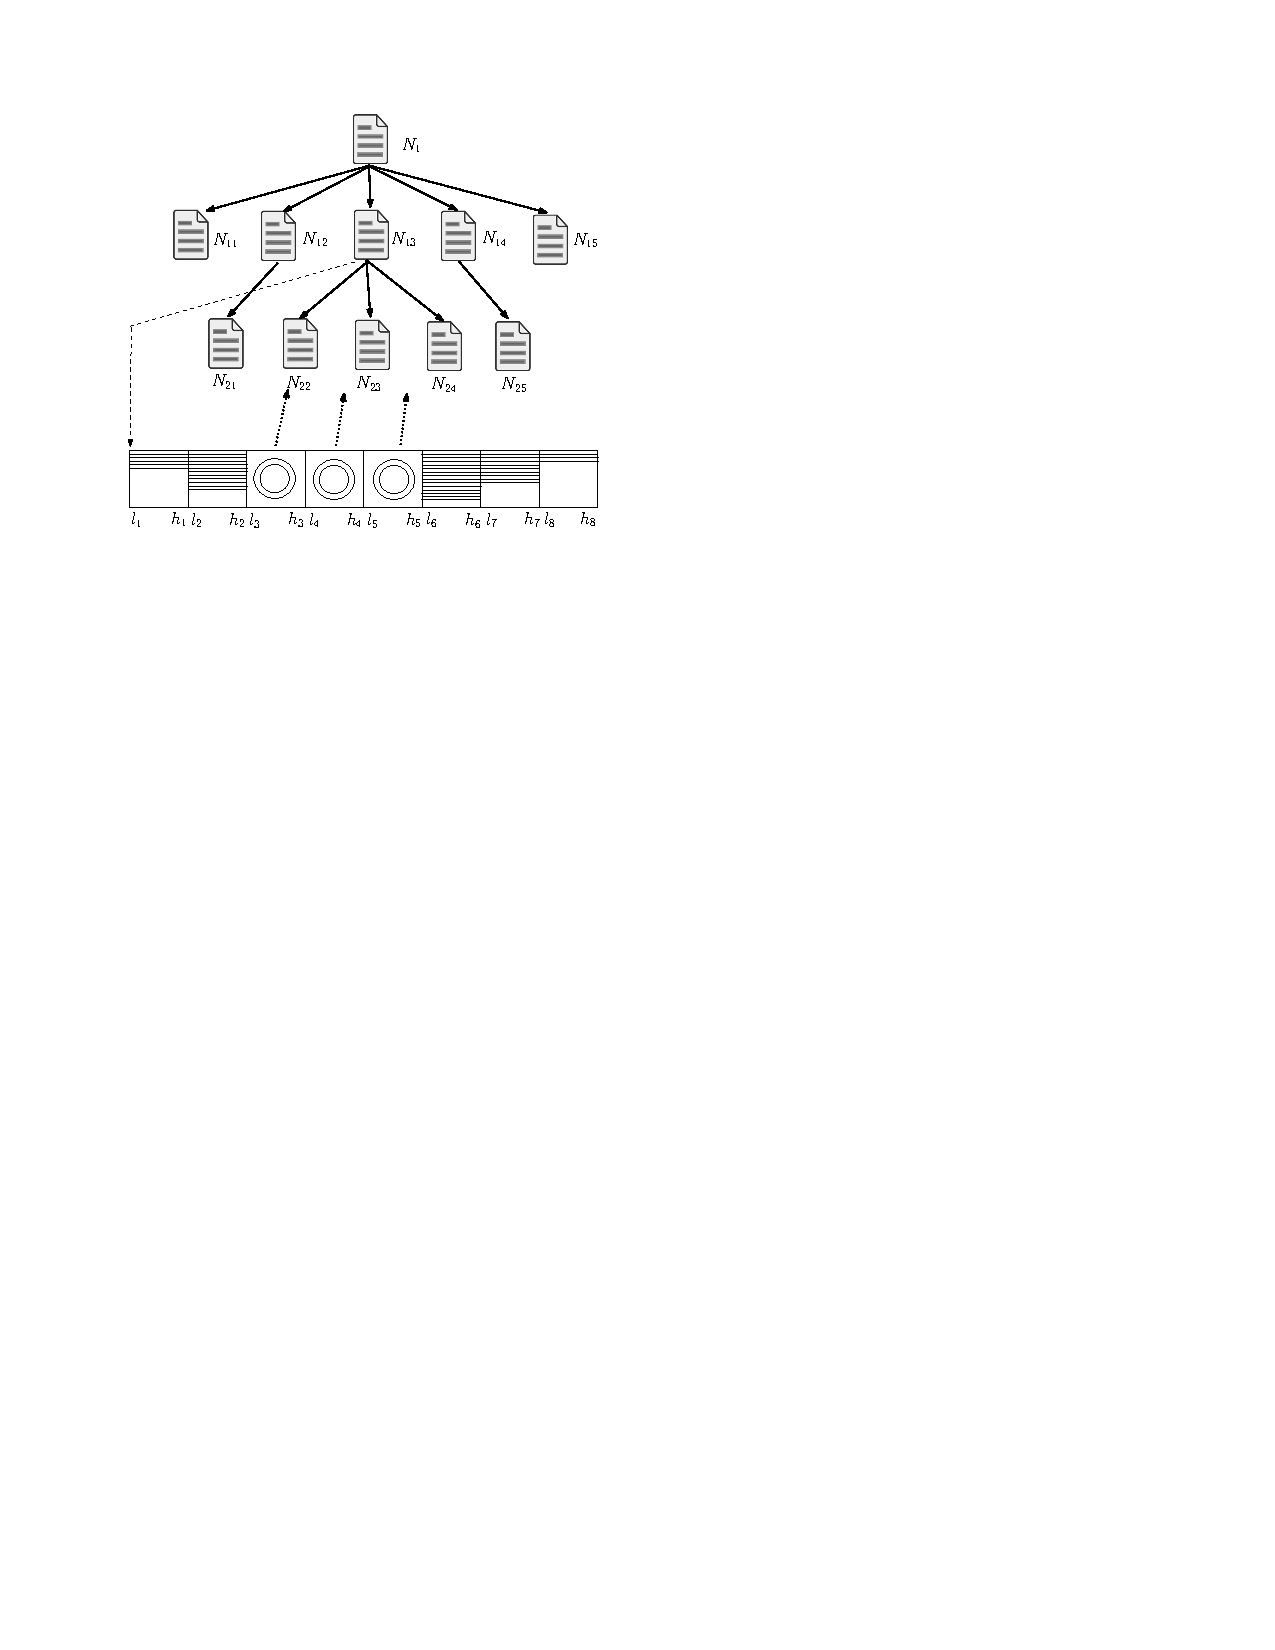
\includegraphics[width=0.65\columnwidth]{chapter2/hashfilestructure.pdf}
\caption{Estrutura del nodo HashFile. Figura adaptada de \cite{lshHashFile}.}
\label{fig:HashFile_structure}
\end{figure}

\newpage
\begin{lstlisting}[mathescape, frame=single, label=alg:HashFile,caption=Consulta kNN aproximada usando HashFile]
algorithm $ApproximateNN$($q, \lambda$)
    $init$ $\delta$
    $\delta$ := $ApproximateNNInNode$($q, root, \delta, \lambda$)
    return $\delta$
end.
procedure [$\delta$] = $ApproximateNNInNode$($q, node, \delta, \lambda$)
    $h_q := node.\textit{hash}(q)$
    for cada nó $child$ do
        $wdist := |child.hash\_value - h_q|$
        if $wdist < \lambda$ then
            insertar $child$ en el $heap$ ordenado por $wdist$
        end if
    end for
    for cada página em disco $p_i$ do
        buscar la lista de paginas de $p_{start}$ a $p_{end}$ en disco entre los intervalor $[h_q - \lambda, h_q + \lambda]$
    end for
    cargar las páginas entre $[h_q - \lambda, h_q + \lambda]$ en el bloque $B$
    for cada objeto $o$ en $B$ do
        $dist := \|o - q\|_{L_2}$
        if dist < $\delta$ then
            $\delta := dist$
        end if
    end for
end.
\end{lstlisting}
\begin{comment}
\begin{lstlisting}[mathescape, frame=single, label=alg:HashFile,caption=Consulta kNN aproximada usando HashFile]
ApproximateNNInNode($q, node, \delta, \lambda$)
    $h_q = node.\textit{hash}(q)$
    for each child node $child$ do
        $wdist = |child.\textit{hash}value - h_q|$
        if $wdist < \lambda$ then
            add child to the heap ordered by $wdist$
    for each disk page $pi$ in increasing order do
        find the list of pages from $p_{start}$ to $p_{end}$ so that their intervals intersect with $[h_q - \lambda, h_q + \lambda]$
    load the $block$ of pages into memory
    for each object $o$ in the $block$ do
        $dist = \|o - q\|_{L_2}$
        if dist < $\delta$ then
            $\delta = dist$
    return $\delta$
end.
ApproximateNN($q, \lambda$)
    init $\delta$
    $\delta$ := ApproximateNNInNode ($q, root, \delta, \lambda$)
    return $\delta$
end.
\end{lstlisting}
\end{comment}

%\begin{figure}[h]
%\centering
% 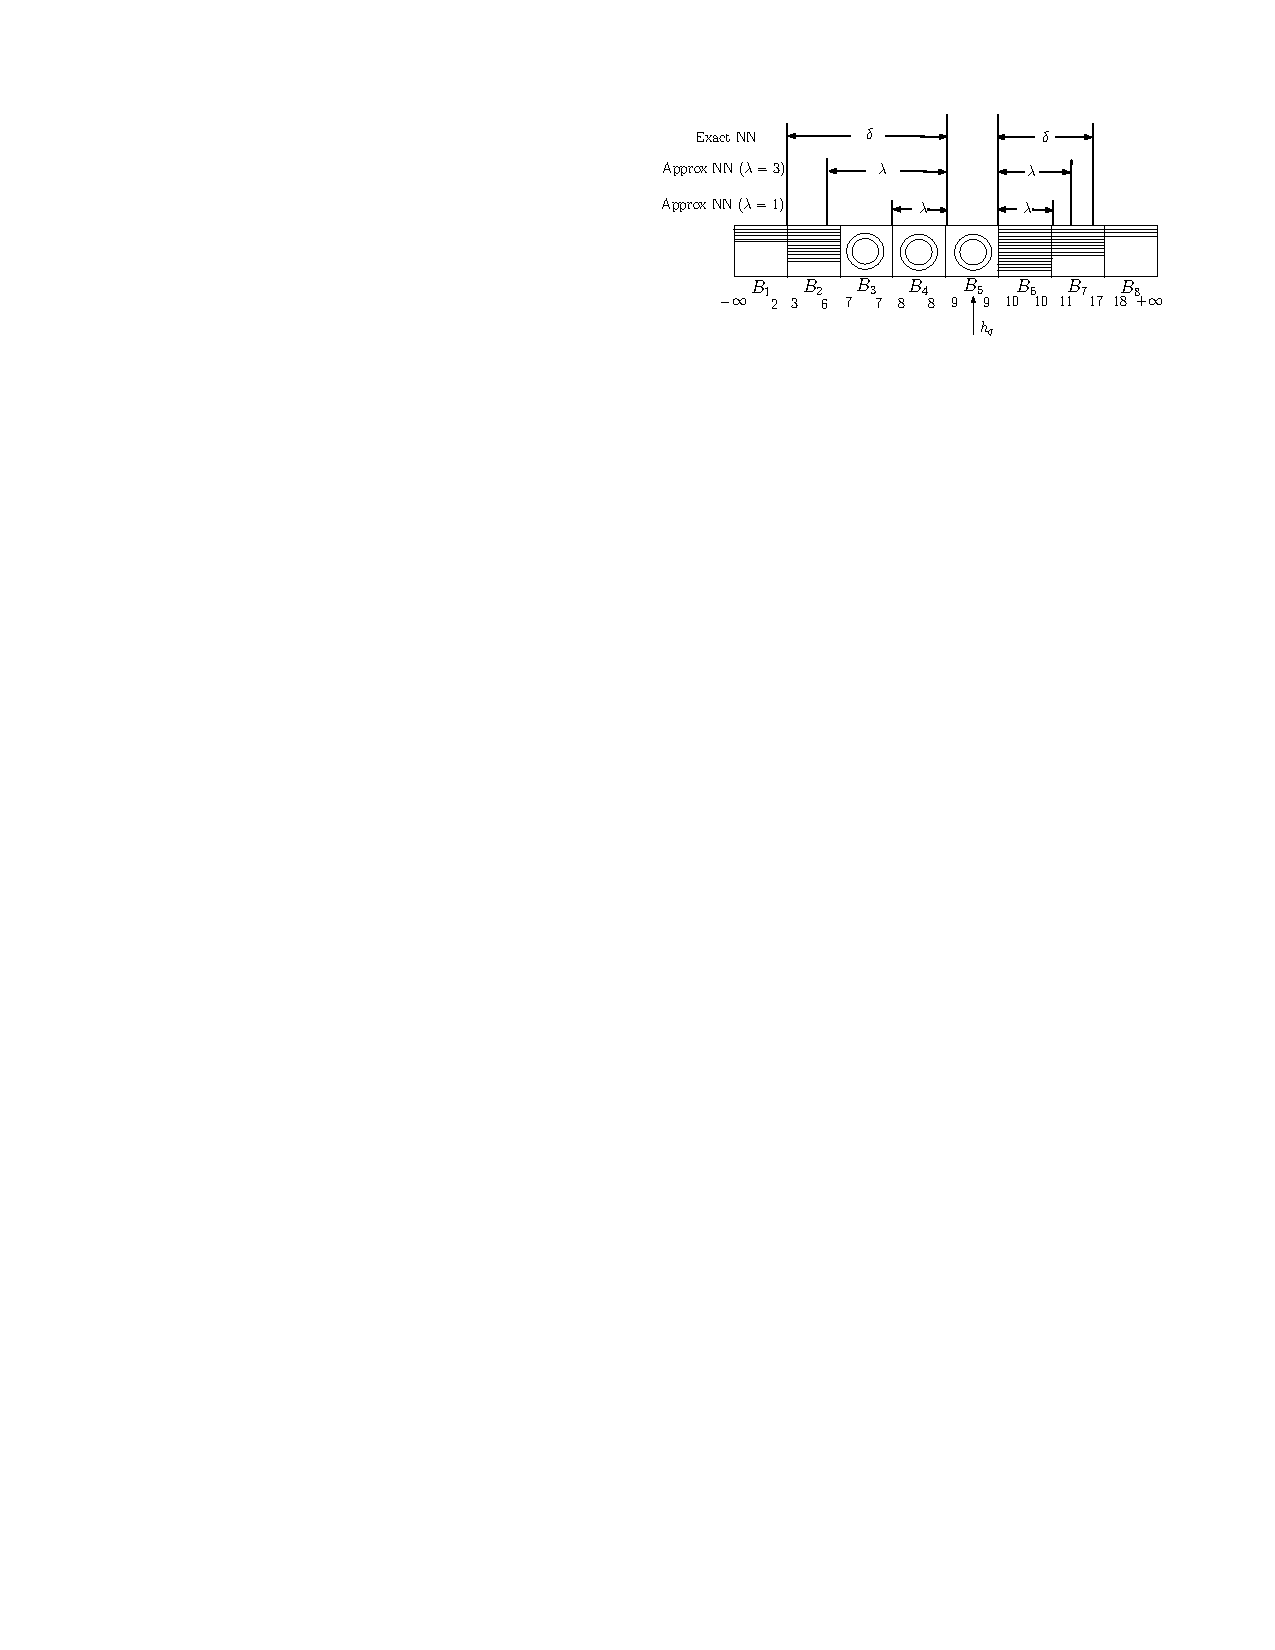
\includegraphics[width=0.7\columnwidth]{chapter2/hashfilequery.pdf}
%\caption{Busca kNN aproximada en un nodo  HashFile.  Figura adaptada de \cite{lshHashFile}.}
%\label{fig:HashFile}
%\end{figure}



\subsubsection{Consulta kNN Aproximada}
 
La Figura \ref{fig:cuda_NN_search} (a) presenta las proyecciones de una consulta por similitud aproximada en Hash-File, donde el objeto de consulta $q$ es mapeado usando las funciones \textit{hash} ($\mathcal{H}_1$ e $\mathcal{H}_2$) en los dos niveles de la estructura. Su estructura lógica correspondiente es presentada en la Figura \ref{fig:cuda_NN_search} (b). En este ejemplo, las proyecciones generan particiones diferentes en el espacio de búsqueda, donde cada función \textit{hash} es utilizada para organizar todo el conjunto de datos, de manera que la proximidad de objetos en el espacio original es mantenida en la proyección. Durante el procesamiento de la consulta, para cada una de las proyecciones el objeto de consulta q es proyectado para el valor \textit{hash} $h_q$, y apenas los objetos dentro del intervalo \textit{hash} $[ h_q - \lambda, h_q + \lambda]$  necesitan ser analizados. De este modo cada nivel contribuye en la precisión de los resultados ampliando el espacio de búsqueda.

\begin{figure}[ht]
 \centering
	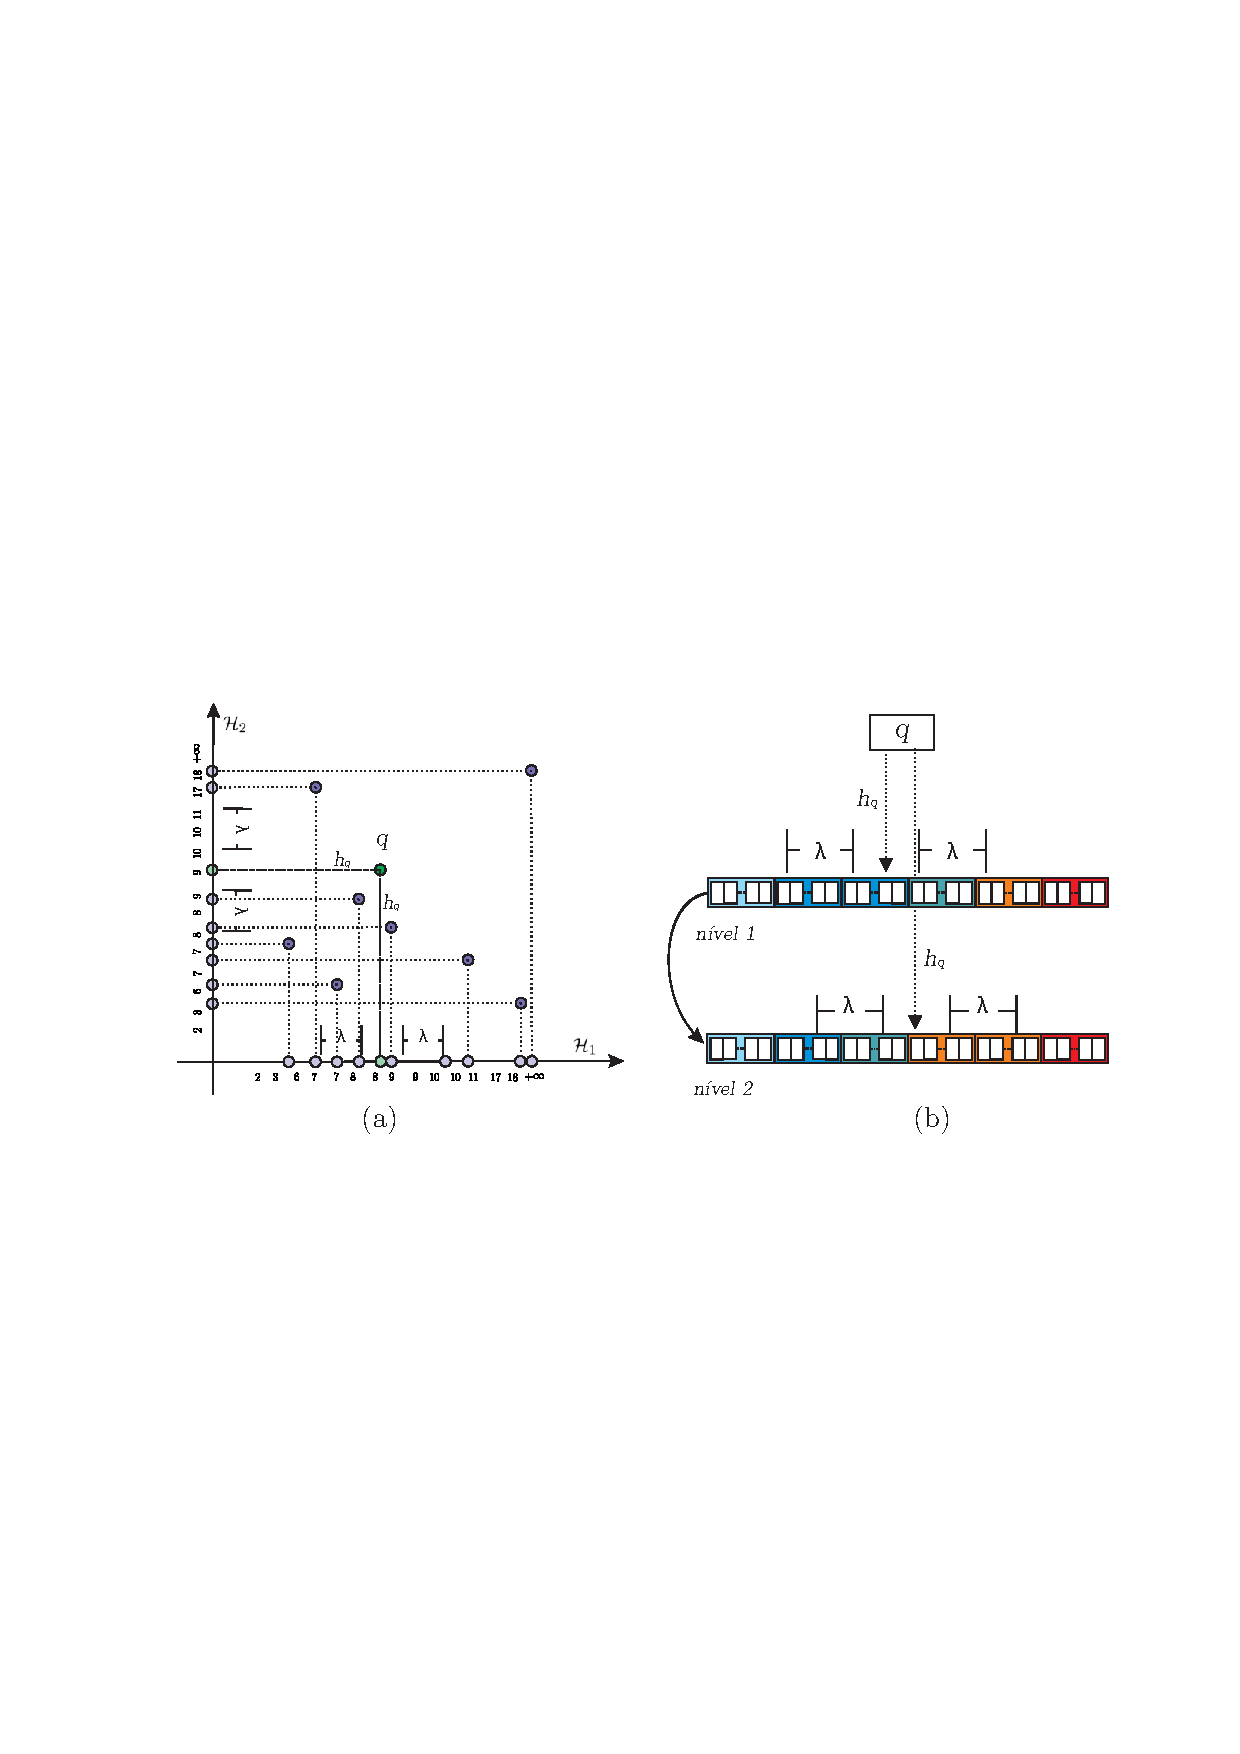
\includegraphics[width=0.99\columnwidth]{chapter2/cuda_hashfile.pdf}
 \caption{Representación de las proyecciones de una consulta por similitud aproximada en HashFile en (a), en (b) se verifica su estructura lógica correspondiente.}
 \label{fig:cuda_NN_search}
\end{figure}
  
Por otro lado, es  sabido que los hiperplanos que generar LSH tienden  poco  poder de discriminación conforme el numero de funciones \textit{hash} crece y además muchas tablas son requeridas para un nivel adecuado de precisión. Esta ineficiencia es debido a su naturaleza de procesamiento de manera independiente a los datos, donde los hiperplanos \textit{hash} son generado sin saber nada sobre la distribución de los datos.  Este problema  ha sido recientemente investigado en muchos métodos basados en \textit{hash} para permitir aprender funciones \textit{hash} adaptadas a la distribución de los datos. Estos métodos serán  discutidas en la siguiente sección. 

%\section{Otros métodos de codificación  para la búsqueda del vecino más cercano}
 
 %% FALTA AQUI UN RESUMEN :(
 
 
\section{Consideraciones Finales}

Como fue discutido en este capitulo,  soluciones exactas para  resolver el problema de búsqueda por similitud en altas dimensiones han sido estudiadas durante años, por otro lado algoritmos probabilísticos han sido poco explorados. De acuerdo con la literatura, es eficiente ejecutar consultas kNN exacta para datos en bajas dimensiones, mas en dimensiones altas las soluciones aproximadas son también una buena opción. El equilibrio entre la eficiencia y la eficacia se vuelve progresivamente más crítico conforme las dimensiones de los datos crece, debido a un fenómeno conocido como   la ``maldición  da la alta dimensionalidad''.

Muchas técnicas exactas y aproximadas, como los Métodos de Acceso Métricos (MAMs) y los métodos basados en \textit{Locality Sensitive Hashing} (LSH) y sus extensiones, fueron propuestas para resolver búsquedas en altas dimensiones.  Entre ellas, los métodos basado en LSH son de las pocas técnicas con garantía teórica de costo sub-linear. No obstante, muchas de sus implementaciones actuales presentan dificultades para ser implementados en problemas reales, como por ejemplo, tareas de minería de datos que dependen de algoritmo de búsqueda al vecino más próximo. He aquí el potencial de los métodos aproximados de búsqueda kNN.

Aún considerando soluciones aproximadas como una vía para mejorar la precisión y desempeño  de las consultas por similitud, problemas como la búsqueda AllkNN en altas dimensiones aun son considerados poco prácticos debido a su alto costo computacional. Estudios recientes, promueven el uso de la \acf{CNN} con técnicas de  \textit{hashing} para mejorar la precisión de la búsqueda de los k-vecinos más cercanos - KNN.  Sin embargo, aun hay retos que resolver para encontrar una solución práctica y eficiente para indexar este tipo de características, como es descrito en el Capitulo 6. 

  
